\documentclass[12pt]{exam}

\newcommand{\course}{MTH 234 Summer 2021}
\newcommand{\qdate}{Cylindrical and Spherical Coordinates} %PUT DATE HERE
\newcommand{\quiz}{Group Work}
 \usepackage{}

    \usepackage[top=1in, bottom=1in, left=.45in, right=.45in]{geometry}
    \usepackage{amsmath,amsthm,amssymb,amstext}
    \usepackage{enumerate,enumitem}
    \usepackage{tikz,float,graphicx}
    \usepackage{microtype}
    \usepackage{bm,tikz}
        \usetikzlibrary{calc,positioning}
    \usepackage{multicol}
    \usepackage{nicematrix}
    \usepackage{cleveref}
    \usepackage[framemethod=tikz]{mdframed}
    \usepackage{graphicx}
    \usepackage[export]{adjustbox}
    
    %\newcommand{\course}{MTH 234 Summer 2021}
    %\newcommand{\qdate}{Equations of lines and planes} %PUT DATE HERE
    %\newcommand{\quiz}{Group Work} 
    
    \newcommand{\R}{\mathbb{R}}
    
    \newcommand{\ba}{\bm{a}}
    \newcommand{\bb}{\bm{b}}
    \newcommand{\bc}{\bm{c}}
    \newcommand{\bi}{\bm{i}}
    \newcommand{\bj}{\bm{j}}
    \newcommand{\bk}{\bm{k}}
    \newcommand{\br}{\bm{r}}
    \newcommand{\bv}{\bm{v}}
    \newcommand{\bu}{\bm{u}}
    \newcommand{\gen}[1]{\left\langle #1 \right\rangle}
    \newcommand{\pd}[2]{\dfrac{\partial #1}{\partial #2}}

\newtheorem*{theorem}{Theorem}
\surroundwithmdframed[]{theorem}

\theoremstyle{definition}
    \newtheorem*{definition}{Definition}
    \surroundwithmdframed[]{definition}
    \newtheorem*{info}{Useful Information}
    \surroundwithmdframed[]{info}
\theoremstyle{remark}
    \newtheorem*{remark}{Remark}
    \surroundwithmdframed[]{remark}
    

%%%%%%%%%%%%%%%%%%%%%%%
% HEADER AND FOOTER
%%%%%%%%%%%%%%%%%%%%%%%
\pagestyle{headandfoot}
\firstpageheadrule
\runningheadrule
\firstpageheader{\course}{\quiz}{\qdate}
\runningheader{\course}{\quiz}{\qdate}
\runningfooter{}{}{}


\usepackage{color}
\shadedsolutions
\definecolor{SolutionColor}{rgb}{0.8,0.9,1}

\usepackage{pgfplots}
    \pgfplotsset{every axis/.append style={
                    axis x line=middle,    % put the x axis in the middle
                    axis y line=middle,    % put the y axis in the middle
                    axis z line=middle,
                    axis line style={<->}, % arrows on the axis
                    xlabel={$x$},          % default put x on x-axis
                    ylabel={$y$},          % default put y on y-axis
                    zlabel={$z$},
                    grid=both,
                    %xtick={-4,...,-1,1,...,3},
                    %ytick={-1,1,}
    }}
    \pgfplotsset{compat=1.17}

\usepackage{pgfplots}
\pgfplotsset{compat = newest}
\newcommand{\bif}{\quad\iff\quad}

\printanswers
%\noprintanswers

\begin{document}

\section*{\qdate}

\subsection*{Cylindrical Coordinates}

\begin{questions}

\question Plot the following points whose cylindrical coordinates are given
    \begin{parts}
    \part \(4,\pi/3,-2\)
    
    \ifprintanswers
        \begin{solution}

            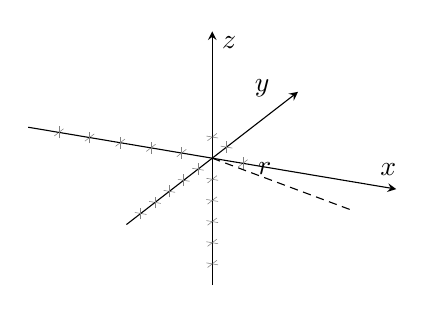
\begin{tikzpicture}
                \begin{axis}[
                    axis lines=center,
                    %view={135}{30},
                    xmin=-6,
                    xmax=6,
                    ymin=-6,
                    ymax=6,
                    zmin=-6,
                    zmax=6,,
                    xtick={-5,...,-1,1,...,5},
                    ytick={-5,...,-1,1,...,5},
                    ztick={-5,...,-1,1,...,5},
                    xticklabel={\empty},
                    yticklabel={\empty},
                    zticklabel={\empty}
                    ]
                    \addplot3[no marks, densely dashed] coordinates 
                    {
                        (0,0,0)
                        (4,1.0472,-2)
                    } node[midway,anchor=south east] {$r$};
                    %\node at (axis cs:)

                \end{axis}
            \end{tikzpicture}

        \end{solution}
    \else
        \vfill
    \fi
    \part \(4,0,2\)
        \ifprintanswers
        \begin{solution}
        \end{solution}
    \else
        \vfill
    \fi
    \end{parts}

\question Convert from rectangular to cylindrical coordinates:
    \begin{parts}
    \part \((-1,1,1)\)
        \ifprintanswers
        \begin{solution}
            \begin{align*}
                r^2 & = x^2+y^2 \\
                    & = (-1)^2+1^2\\
                    & = 2
            \end{align*}
            So
            \[
                r^2 = 2 \bif r=\pm\sqrt{2}
            \]
            And from 
            \begin{align*}
                \tan\theta = \frac{y}{x}
                            = -1
            \end{align*}
            we get 
            \[
                \theta = \tan^{-1}(-1) = \frac{3\pi}{4}
            \]
            So in cylindrical coordinates the point is \(\sqrt{2},3\pi/4,1\).
        \end{solution}
    \else
        \vfill
    \fi
        \part \((-2,2\sqrt{3},3)\)
        \ifprintanswers
        \begin{solution}
            \[
                (4,2\pi/3,3)
            \]
        \end{solution}
    \else
        \vfill
    \fi
    \end{parts}

\question Convert from cylindrical coordinates to rectangular coordinates
    \begin{parts}
        \part  \((4,\pi/3,-2)\)
        \ifprintanswers
        \begin{solution}
            \[
                \tan(\pi/3)=\frac{y}{x} \bif \sqrt{3}=\frac{y}{x}\bif \sqrt{3}x=y
            \]
            and
            \[
                r^2=x^2+y^2\bi 16=x^2+(\sqrt{3}x)^2 \bif 16=4x^2 \bif \(x=\pm2\)
            \]
            From the position of the angle \(\pi/3\) we obtain
            \[
                (2,2\sqrt{3},-2).
            \]
        \end{solution}
    \else
        \vfill
    \fi
        \part \((4,0,2)\)
        \ifprintanswers
        \begin{solution}
            The point in cartesian coordinates is also expressed by 
            \[
                \(4,0,2\).
            \]
        \end{solution}
    \else
        \vfill
    \fi
    \end{parts}
\newpage

\question Sketch the solid described by the following
    \begin{parts}
        \part 
            \[
                0\le r\le 2,\quad -\pi/2\le \theta\le \pi/2,\quad 0\le z\le 1
            \]
        \ifprintanswers
        \begin{solution}
            
        \end{solution}
    \else
        \vfill
    \fi
        \part 
        \[
            0 \le \theta \le \pi/2,\quad r\le z \le 2
        \]
        \ifprintanswers
        \begin{solution}
        \end{solution}
    \else
        \vfill
    \fi
    \end{parts}
\question Describe in words or draw a rough sketch of the surface whose equation is given
    \begin{parts}
        \part \(\theta=\pi/4\)
        \ifprintanswers
        \begin{solution}
        \end{solution}
    \else
        \vfill
    \fi
        \part \(r=15\)
        \ifprintanswers
        \begin{solution}
        \end{solution}
    \else
        \vfill
    \fi 
        \part \(z=4-r^2\)
        \ifprintanswers
        \begin{solution}
        \end{solution}
    \else
        \vfill
    \fi
        \part \(2r^2+z^2=1\)
        \ifprintanswers
        \begin{solution}
        \end{solution}
    \else
        \vfill
    \fi
    \end{parts}
\question Convert the given equation to cylindrical coordinates
    \begin{parts}
        \part \(x^2-4x+y^2+z^2=1\)
        \ifprintanswers
        \begin{solution}
        \end{solution}
    \else
        \vfill
    \fi
        \part \(z=x^2-y^2\)
        \ifprintanswers
        \begin{solution}
        \end{solution}
    \else
        \vfill
        \newpage
    \fi
    \end{parts}


\subsection*{Spherical Coordinates}

\question Plot the following points whose spherical coordinates are given then find the rectangular coordinates for the same point.
    \begin{parts}
        \part \((6,\pi/3,\pi/6)\)
        \ifprintanswers
        \begin{solution}
        \end{solution}
    \else
        \vfill
    \fi
        \part \((3,\pi/2,3\pi/4)\)
        \ifprintanswers
        \begin{solution}
        \end{solution}
    \else
        \vfill
    \fi
    \end{parts}

\question Convert from rectangular to spherical coordinates:
    \begin{parts}
        \part \((0,-2,0)\)
        \ifprintanswers
        \begin{solution}
        \end{solution}
    \else
        \vfill
    \fi
        \part \((1,0,\sqrt{3})\)
        \ifprintanswers
        \begin{solution}
        \end{solution}
    \else
        \vfill
        \newpage
    \fi
    \end{parts}
    



\question Identify or describe in words or sketch the surface whose equation is given
    \begin{parts}
        \part \(\rho=3\)
        \ifprintanswers
        \begin{solution}
        \end{solution}
    \else
        \vfill
    \fi
        \part \(\rho=\sin\theta\sin\phi\)
        \ifprintanswers
        \begin{solution}
        \end{solution}
    \else
        \vfill
    \fi 
    \end{parts}
\question Write the equation in spherical coordinates
    \begin{parts}
        \part \(z^2=x^2+y^2\)
        \ifprintanswers
        \begin{solution}
        \end{solution}
    \else
        \vfill
    \fi
        \part \(x+2y+3z=1\)
        \ifprintanswers
        \begin{solution}
        \end{solution}
    \else
        \vfill
    \fi
        \part \(x^2+z^2=9\)
        \ifprintanswers
        \begin{solution}
        \end{solution}
    \else
        \vfill
    \fi
    \end{parts}

\end{questions}

\end{document}

% soln : Question environment
    \ifprintanswers
        \begin{solution}
        \end{solution}
    \else
        \vfill
    \fi